%# -*- coding:utf-8 -*-
% Author: Guang Touge, PhilFan
% Date: 2025-07-10

\PassOptionsToPackage{quiet}{fontspec} 
\documentclass[10pt,aspectratio=169,mathserif]{beamer}		
%设置为 Beamer 文档类型,设置字体为 10pt,长宽比为16:9,数学字体为 serif 风格

\usepackage{zju_beamer}
\setCJKmainfont{PingFang SC} % Mac 系统默认字体,Mac 用户取消注释
% \setCJKsansfont{FandolHei} % 设置中文无衬线字体
% \setCJKmonofont{FandolHei} % 设置等宽字体为黑体
\graphicspath{{./figures/}} % 指定图片所在文件夹  

\beamertemplateballitem		%设置 Beamer 主题


% 首页信息设置
\title[浙江大学 Beamer 模板]{浙江大学 Beamer 模板}
\subtitle{——这里是副标题}
\author[Guang Touge, PhilFan]{光头哥, PhilFan}
\institute[IOPP]{计算机学院 \\ 浙江大学}
\date{\today}




\begin{document}

\begin{frame}
	\titlepage
\end{frame}				%生成标题页

\section{提纲}
\begin{frame}
	\frametitle{提纲}
	\tableofcontents
\end{frame}				%生成提纲页

\section{介绍}
\begin{frame}
	\frametitle{介绍}

	\begin{itemize}
		\item {编译方式}
		      \begin{itemize}
			      \item  推荐安装完整版的 TeXLive
			      \item 使用 \XeLaTeX 编译
		      \end{itemize}
		\item 请参考 \LaTeX 和 Beamer 用户文档

		\item 行内数学公式示例 $\sin^2 \theta + \cos^2 \theta = 1$
		\item {行间数学公式示例 \begin{equation}
			      y_{1}=\int \sin x\, {\rm d}x
		      \end{equation}	 }
		\item 基于“浙大蓝”颜色 \url{https://www.zju.edu.cn/}
	\end{itemize}
\end{frame}

\section{内置环境}
\begin{frame}{内置环境}{副标题}
	\begin{block}{Slides with \LaTeX}
		Beamer offers a lot of functions to create nice slides using \LaTeX.
	\end{block}

	\begin{block}{The basis}
		内部使用以下主题
		\begin{itemize}
			\item split
			\item whale
			\item rounded
			\item orchid
		\end{itemize}
	\end{block}
\end{frame}

\begin{frame}
	\frametitle{带数字列表}
	\begin{enumerate}
		\item This just shows the effect of the style
		\item It is not a Beamer tutorial
		\item Read the Beamer manual for more help
		\item Contact me only concerning the style file
	\end{enumerate}
\end{frame}

\begin{frame}{并排图片显示}
可以通过minipage的方式实现并排效果,比如图片排版:
	\begin{figure}[ht]
		\centering
		% 第一张图片
		\begin{minipage}[b]{0.45\linewidth} % 使用 45% 的行宽
			\centering
			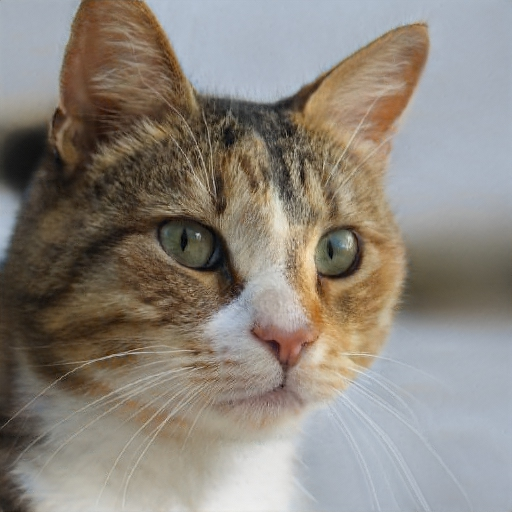
\includegraphics[width=0.5\linewidth]{example.png}
			\caption{第一张图片标题}
			\label{fig:image1}
		\end{minipage}
		\hfill % 在两个 minipage 之间添加一些水平空间
		% 第二张图片
		\begin{minipage}[b]{0.45\linewidth} % 使用 45% 的行宽
			\centering
			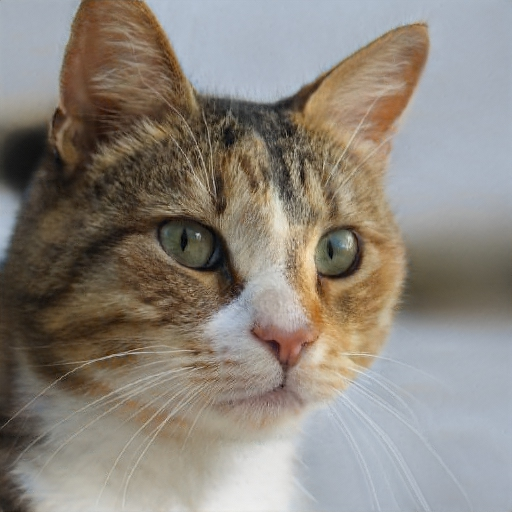
\includegraphics[width=0.5\linewidth]{example.png}·
			\caption{第二张图片标题}
			\label{fig:image2}
		\end{minipage}
	\end{figure}
\end{frame}
	

\begin{frame}[fragile]
\frametitle{示例代码}
\begin{lstlisting}[language=C++]
#include <iostream>

class HelloWorld {
public:
    void sayHello() {
        std::cout << "Hello, World!" << std::endl;
    }
};

int main() {
    HelloWorld hw;
    hw.sayHello();
    return 0;
}
\end{lstlisting}
\end{frame}

\section{结论}
\begin{frame}
	\frametitle{结论}

	\begin{itemize}
		\item Easy to use
		\item Good results
	\end{itemize}
\end{frame}

\section{参考文献}
\begin{frame}[allowframebreaks]%实现自动分页
    \frametitle{参考文献}
    \reference
\end{frame}

\end{document}